% Generated from journal.tex by tools/prepare_jss.py.
\documentclass[preprint,12pt]{elsarticle}
\usepackage{lmodern}
\usepackage[T1]{fontenc}
\usepackage{amsmath,amssymb,amsthm,microtype}
\usepackage{booktabs,tabularx,array,graphicx,xcolor}
\usepackage{tikz}
\usetikzlibrary{positioning,arrows.meta,fit}
\usepackage[hidelinks]{hyperref}
\usepackage{xurl}
\newtheorem{theorem}{Theorem}
\newtheorem{proposition}[theorem]{Proposition}
\newtheorem{lemma}[theorem]{Lemma}
\theoremstyle{definition}\newtheorem{definition}[theorem]{Definition}
\newcommand{\PASS}{\mathsf{PASS}}\newcommand{\FAIL}{\mathsf{FAIL}}\newcommand{\UNKNOWN}{\mathsf{UNKNOWN}}
\newcommand{\E}{\mathbb E}\newcommand{\ind}{\mathbf 1}
\DeclareMathOperator*{\argmin}{arg\,min}
\setlength{\emergencystretch}{2em}

\makeatletter
\def\ps@pprintTitle{\let\@oddhead\@empty\let\@evenhead\@empty
\def\@oddfoot{\hfil\thepage\hfil}\let\@evenfoot\@oddfoot}
\makeatother
\hypersetup{pdftitle={Adaptive HACT: Information Limits and Safe Adaptation of Verification Evidence},pdfauthor={}}
\journal{Journal of Systems and Software}
\begin{document}
\begin{frontmatter}
\title{Adaptive HACT: Information Limits and Safe Adaptation of Verification Evidence}
\author{Anonymous authors}
\begin{abstract}
Adaptive verification evidence raises two questions: which completion
statistics identify an efficient representation, and how may that
representation change without weakening acceptance? Adaptive HACT
(Hyperedge-Aware Certificate Trees) separates a protected semantic registry
from generation-fenced certificate trees and prices packets touched by joint
completion sets. We prove that exact singleton and pairwise probabilities
can leave globally optimal trees unidentified for every fanout of at least
three and every affine positive-slot packet price, with sharp minimax
regret. A complete-epoch construction extends this limitation to fixed-eight
batching within a two-layout class. Under exchangeable complete batches, a
specialization of established tree optimization provides an exact global
baseline. A local publication invariant preserves acceptance through
migration; a conditional adoption rule includes calibration, shift and
installation costs. Independent enumeration checks 74,245 tree comparisons.
Retrospective scoring finds that the symmetric baseline beats frozen
full-wave refinement on all 15 item-shuffled traces and loses on all 15
file-group traces. It costs 21.26--62.13\% more on original holdouts.
Without byte observers, the tree service takes 1.61--3.54 times the
maintained-counter ledger's operation time. The results establish
information limits and conditional adaptation guarantees; service and agent
speedups remain unproven.
\end{abstract}
\begin{keyword}
Verification evidence \sep software agents \sep completion hypergraphs \sep adaptive data structures \sep runtime assurance
\end{keyword}
\end{frontmatter}
\section{Introduction}
Software agents navigate repositories, run checks and revise candidates
over trajectories much longer than a single generated patch. Repository
benchmarks and systems such as SWE-bench, SWE-agent and OpenHands make
the interaction between generation and tooling observable~\cite{swebench,sweagent,openhands}.
Verification-first approaches additionally bind consequential actions to
checkable evidence~\cite{aiware,traceassurance}. These systems create an
infrastructure question even when the checker and acceptance criteria are
already fixed: how may an orchestrator reorganize accumulated evidence
without changing what that evidence authorizes?

Operators may inspect incomplete coverage, locate failures, replay completion
batches and request bounded diagnostic pages. An indexed ledger can already
provide these services; a hierarchy must repay construction, maintenance and
adaptation. Optimizing a prescribed packet format also requires justifying
that format's consumer utility.

Adaptive HACT (Hyperedge-Aware Certificate Trees) separates a protected
semantic registry from a replaceable certificate tree. Acceptance requires
current trusted records for all declared checks; advisory layouts change
only representation. A monotone generation fences publication tickets
through migration, including a return to an earlier layout.

The representation objective depends on completion \emph{sets}. If several
checks finish before a refresh, an internal packet is emitted once whenever
its coverage intersects that set. Pairwise co-activity is convenient for
ordering leaves, but can omit the higher-order event that determines whether
a larger subtree is touched. Our main theoretical result goes beyond
showing different costs for one chosen subtree: it constructs identical
pairwise observations with disjoint globally optimal trees for an entire
family of packet prices and fanouts. A sharp minimax penalty quantifies
what even exact pairwise information cannot recover.

The fixed-eight extension shows that this obstruction also affects a
specified local refinement decision when every check completes exactly once;
it does not promote the embedded layouts to global optima. Table~\ref{tab:novelty}
separates these claims from the established ingredients.

The obstruction disappears under a declared symmetry model. If a uniform
completion permutation is divided into fixed batch sizes, expected packet
cost depends only on coverage cardinality. A size-state dynamic program
then optimizes all shapes and permutations exactly in $O(bn^2)$ arithmetic
operations after computing the cardinality weights. This model-specific instance of established batch-update tree
optimization~\cite{graham2007} is a stronger null baseline than one compact
topology: when the future law remains exchangeable conditional on training,
learning cannot improve its expected cost.

The practical question remains empirical. A compiler that retains full
waves may still offer little improvement over a compact balanced tree.
A hierarchical service may also lose to a ledger with maintained counters.
We test both possibilities without using an analytical separation as
evidence of an execution speedup. The paper makes four contributions:
\begin{enumerate}
\item A conditional local invariant separating acceptance semantics from
adaptive evidence layouts, including stable identities, conflicts and
generation-fenced migration.
\item A packet-refresh model and a parameter-general information lower
bound with sharp deterministic and randomized pairwise-only regret,
plus a fixed-batch candidate-class separation.
\item An exact global reference under exchangeable complete batches,
contrasted with bounded full-wave refinement for structured observations;
a conditional adoption rule uses paired-cost bounds, calibration
uncertainty and installation amortization.
\item A reproducible evaluation distinguishing historical representation
results, new upstream test executions and controlled service demand, with
strong ledger controls and explicit resource failures.
\end{enumerate}
Classical alphabetic optimization, clustering, caching and expert selection
remain established ingredients. We make no priority claim for the general
use of hyperedges or hierarchies. Our claim concerns their explicit
composition under the stated verification contract and packet objective.

\begin{figure*}[t]
\centering
\resizebox{\textwidth}{!}{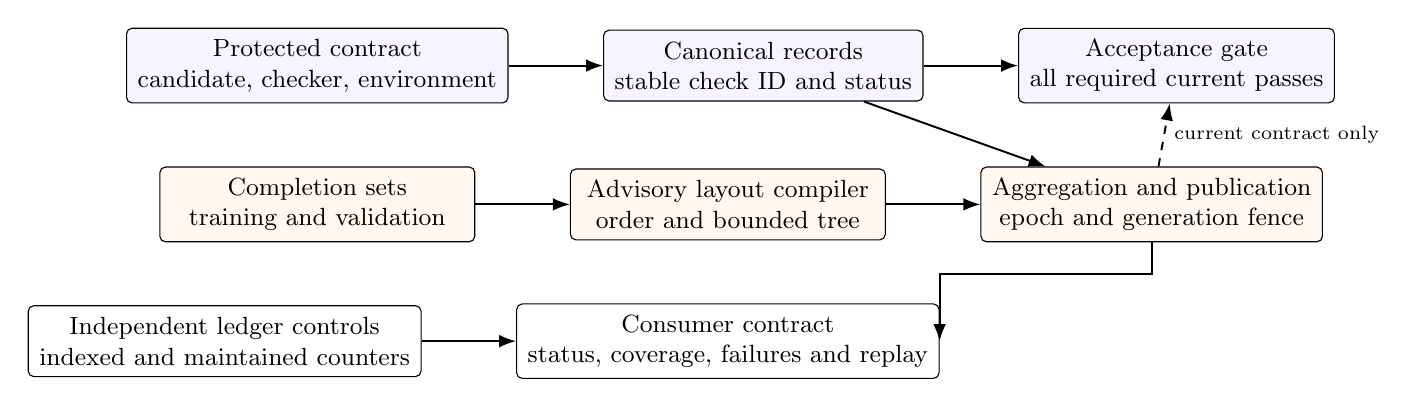
\begin{tikzpicture}[
 >=Latex,box/.style={draw,rounded corners=2pt,align=center,minimum height=9mm,minimum width=40mm,inner sep=4pt,font=\small},
 sem/.style={box,fill=blue!4},lay/.style={box,fill=orange!6},
 arr/.style={->,line width=.7pt},node distance=8mm and 12mm]
 \node[sem] (contract) {Protected contract\\candidate, checker, environment};
 \node[sem,right=of contract] (records) {Canonical records\\stable check ID and status};
 \node[sem,right=of records] (gate) {Acceptance gate\\all required current passes};
 \draw[arr] (contract)--(records);\draw[arr] (records)--(gate);
 \node[lay,below=of contract] (waves) {Completion sets\\training and validation};
 \node[lay,right=of waves] (layout) {Advisory layout compiler\\order and bounded tree};
 \node[lay,right=of layout] (kernel) {Aggregation and publication\\epoch and generation fence};
 \draw[arr] (waves)--(layout);\draw[arr] (layout)--(kernel);
 \draw[arr] (records)--(kernel);
 \draw[arr,dashed] (kernel)--node[right,font=\scriptsize]{current contract only}(gate);
 \node[box,below=of layout] (service) {Consumer contract\\status, coverage, failures and replay};
 \draw[arr] (kernel.south)--++(0,-4mm)-|(service.east);
 \node[box,left=of service] (ledger) {Independent ledger controls\\indexed and maintained counters};
 \draw[arr] (ledger)--(service);
\end{tikzpicture}}
\caption{Semantic authority, adaptive representation and the consumer contract.
The compiler cannot modify the protected contract or canonical outcomes.
Both ledger controls and the tree answer the same diagnostic requests.
The diagram is rendered from the included TikZ source; AI assistance is
disclosed in the acknowledgments.}
\label{fig:journal-architecture}
\end{figure*}

\section{Model and Measurement Contract}\label{sec:jmodel}
Let $\mathcal R=(g_0,\ldots,g_{n-1})$ be a nonempty registry of unique semantic
check IDs. A candidate identity
$e=(\mathrm{epoch},\mathrm{snapshot},\mathrm{checker},\allowbreak
\mathrm{environment},\mathrm{registry})$
binds the source and protected acceptance inputs. The epoch increases even
after a return to identical source bytes. Only a trusted runner can supply
final $\PASS$, $\FAIL$ or $\UNKNOWN$ records. Missing, stale, skipped,
incompatible or timed-out evidence does not count as a pass.

A layout $L=(\pi,T)$ maps leaf positions through an exact permutation $\pi$
of semantic indices. Each internal node's children partition its positional
interval without overlap or omissions. Its semantic coverage is $G_L(v)$.
Check execution order is independent of layout order. The acceptance
predicate is, with $E_e(g_i)$ denoting the current matching trusted status,
\begin{equation}\label{eq:accept}
 A(e)=\prod_{g_i\in\mathcal R}\ind\{E_e(g_i)=\PASS\}.
\end{equation}
An observed failure permits rejection before the remaining checks execute,
but supplies no evidence for the unexecuted remainder.

An internal node with $d$ children emits a packet costing
\begin{equation}\label{eq:packet}
 c(d)=H+Sd,\qquad 2\le d\le
 b=\left\lfloor(C-H)/S\right\rfloor.
\end{equation}
The implementation uses $H=512$, $S=320$, $C=3072$ bytes and $b=8$.
Mandatory fields exceeding their slots are rejected. The cap is per packet;
registry manifests are separate control artifacts whose bytes must be charged.

Let $U_{e,a}$ contain the semantic indices whose final records arrive
between two refreshes. The strict-epoch padded cost is
\begin{equation}\label{eq:jcost}
 \ell_e(L)=W(L)+\sum_a\sum_{v\in\operatorname{int}(T)}
 c(d_v)\ind\{G_L(v)\cap U_{e,a}\ne\varnothing\},
\end{equation}
where $W(L)=\sum_vc(d_v)$ constructs an initially unknown tree.
We call $U_{e,a}$ a completion hyperedge. This model charges the full initial
tree and every touched ancestor, rather than using independent activation
probabilities. Persistent refresh models omit a cold build at each event;
each actual installation is still cold and priced.

A layout switch from $i$ to $j$ additionally costs
$M_{ij}=|\mathrm{manifest}(L_j)|+W(L_j)$ when layouts differ.
This is the evaluated uncompressed installation protocol, not a universal
network cost. A format using compression or deltas defines a different
objective and needs its own measurements. Padded packets, compressed
archives, answer traffic, serialized state, RAM and elapsed time remain
separate units.

\section{An Information Limit of Pairwise Summaries}
\begin{proposition}[Pairwise probabilities omit subtree-hit information]\label{prop:pairwise}
On three leaves, let $P$ be uniform on
$\varnothing,\{0,1\},\{0,2\},\{1,2\}$ and $Q$ uniform on
$\{0\},\{1\},\{2\},\{0,1,2\}$. Both have singleton probabilities $1/2$,
pairwise joint probabilities $1/4$ and Jaccard affinities $1/3$, but the
triple is touched with probabilities $3/4$ and $1$.
\end{proposition}
This parity fact alone does not imply different global optima: another tree
might dominate in both worlds. The following theorem rules that out under
the affine packet objective.
\begin{theorem}[Pairwise information has a sharp optimization penalty]\label{thm:pairwise-optimum}
Let $b\ge3$ be an integer, $H\ge0$, $S>0$, and $\lambda\ge0$.
For $n=b+1$ labeled leaves and internal arities $2,\ldots,b$, define
\begin{align*}
 J_D(T;\lambda)&=\lambda W(T)\\
 &\quad+\E_{U\sim D}\sum_{v\in\operatorname{int}(T)}c(d_v)
       \ind\{G(v)\cap U\ne\varnothing\}.
\end{align*}
There are distributions $P,Q$ with identical singleton and pairwise
probabilities but disjoint globally optimal tree sets, over every feasible
shape and leaf permutation. With $W_2=2H+S(b+2)$,
\begin{align}
 J_P^*&=(1+\lambda)W_2-(H+3S)/4,\label{eq:general-p}\\
 J_Q^*&=(1+\lambda)W_2-(H+2S)/4.\label{eq:general-q}
\end{align}
Any deterministic selector observing only those exact pairwise summaries has
worst-case regret at least $S/4$. The sharp randomized minimax regret is
\begin{equation}\label{eq:minimax-pairwise}
 \frac{S(H+2S)}{4(H+3S)}.
\end{equation}
Sibling orders are treated as equivalent.
\end{theorem}
\begin{proof}
Append $b-2$ anchor leaves, present in every event, to the two three-leaf
parity laws of Proposition~\ref{prop:pairwise}. Every singleton and pairwise
probability agrees, including anchor/parity pairs. An anchor-containing
node is always touched; a node containing only parity leaves is touched
with probability at least $3/4$.

If $I$ is the number of internal nodes, edge counting gives
$W(T)=I(H+S)+Sb$, and the arity cap implies $I\ge2$.
At most two internal nodes contain only the three parity leaves. If there
are two, both are binary; if there is one, its arity is at most three.
Their total price is at most $2c(2)$. Thus for either law and $I\ge3$,
\[
 J_D(T;\lambda)\ge(1+\lambda)W(T)-c(2)/2.
\]
A tree with two internal nodes and a parity-pair child costs
$(1+\lambda)W_2-c(2)/4$ under either law. Every $I\ge3$ lower bound exceeds
that pair tree by at least
\[
 (1+\lambda)(H+S)-c(2)/4
 = (3H+2S)/4+\lambda(H+S)>0.
\]
Such trees are componentwise dominated. With $I=2$, a child containing an
anchor is also dominated by a parity pair. The remaining choices are a
parity pair or the full parity triple. A pair is missed with probability
$1/4$ under either law. The triple is missed with probability $1/4$ under
$P$ and zero under $Q$. Since $c(3)>c(2)$, $P$ uniquely chooses the triple,
whereas $Q$ chooses any of its three pairs. This proves
Equations~\eqref{eq:general-p}--\eqref{eq:general-q}, including construction.

A pairwise-only rule receives identical inputs in both worlds. All other
tree classes are dominated, so a randomized rule need only choose the triple
with probability $q$ and a pair otherwise. Its two regrets are
\[
 r_P(q)=S(1-q)/4,\qquad r_Q(q)=(H+2S)q/4.
\]
The best deterministic choice is a pair, giving worst-case regret $S/4$.
Equating the two affine regrets gives $q^*=S/(H+3S)$ and
Equation~\eqref{eq:minimax-pairwise}. This mixture attains the lower bound.
\end{proof}

The result covers every affine positive-slot price and every fanout at least
three; it is not specific to the artifact's selected byte constants. It
concerns an interface exposing exact population pairwise summaries.
It does not assert equivalence of finite-sample statistical experiments:
joint fluctuations of empirical summary vectors can retain higher-order
information. It neither bounds a method
that retains full waves nor establishes the prevalence of such laws in
software executions. The events describe persistent refresh; a partial
event is not asserted to be a complete strict verification epoch.

\begin{figure}[t]\centering
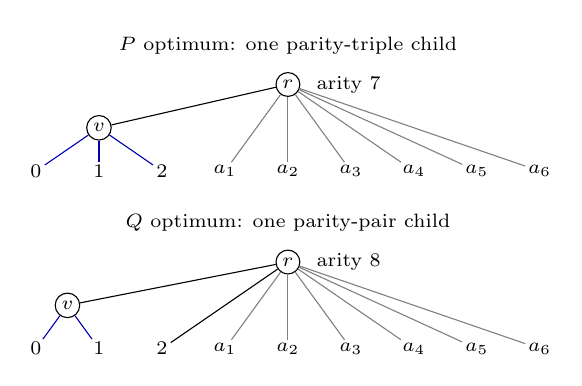
\begin{tikzpicture}[x=.8cm,y=.55cm,every node/.style={font=\scriptsize},
 root/.style={circle,draw,inner sep=1.3pt}, leaf/.style={inner sep=1pt}]
\node at (4,2.9) {$P$ optimum: one parity-triple child};
\node[root] (pr) at (4,2) {$r$};
\node[root] (pt) at (1,1) {$v$};
\node[right] at (4.3,2) {arity 7};
\foreach \x/\lab in {0/0,1/1,2/2,3/a_1,4/a_2,5/a_3,6/a_4,7/a_5,8/a_6}{
 \node[leaf] (p\x) at (\x,0) {$\lab$};}
\draw (pr)--(pt);
\foreach \x in {0,1,2}{\draw[blue!70!black] (pt)--(p\x);}
\foreach \x in {3,...,8}{\draw[gray] (pr)--(p\x);}
\node at (4,-1.2) {$Q$ optimum: one parity-pair child};
\node[root] (qr) at (4,-2.1) {$r$};
\node[root] (qt) at (.5,-3.1) {$v$};
\node[right] at (4.3,-2.1) {arity 8};
\foreach \x/\lab in {0/0,1/1,2/2,3/a_1,4/a_2,5/a_3,6/a_4,7/a_5,8/a_6}{
 \node[leaf] (q\x) at (\x,-4.1) {$\lab$};}
\draw (qr)--(qt);
\foreach \x in {0,1}{\draw[blue!70!black] (qt)--(q\x);}
\draw (qr)--(q2);
\foreach \x in {3,...,8}{\draw[gray] (qr)--(q\x);}
\end{tikzpicture}
\caption{Nine-leaf witness for Theorem~\ref{thm:pairwise-optimum}, with
$H=512,S=320,b=8$. The six anchors $a_i$ are distinct always-present
leaves, each a separate root child. Grouping the parity triple costs
3,856/4,224 refresh bytes under $P/Q$; grouping a pair costs 3,936
under either law. Construction adds 4,224 bytes to both trees.}
\label{fig:pairwise-witness}
\end{figure}


At these prices the deterministic penalty is 80 bytes; randomized minimax
regret is $1440/23\simeq62.609$ bytes, attained by choosing the triple with
probability $5/23$. Integer byte counts are the implementation case; the
theorem also allows real prices. Its zero-header boundary does not change
the serializer's stricter positive-header validation.

An independently implemented exact rational reference checks 39 parameter
cases, including zero headers, fractional construction and header-dominated
prices. It imports no HACT objective or optimizer. The nine-leaf case visits
511 nonempty subset subproblems and 115,462 candidate partitions \emph{across
those subproblems}; it finds one $P$ optimum and three $Q$ optima. Twenty-three
tests include independently listed four-leaf trees and deliberate formula
corruption. These are analytical checks, not additional software workloads.

\subsection{The separation also occurs in complete epochs}
Persistent refresh is not the only affected regime. Complete epochs
partition all obligations into disjoint nonempty waves.
\begin{theorem}[Complete-epoch information separation]\label{thm:strict-pairwise}
For any fanout $b\ge6$, $S>0$ and $16/11<H/S<28/17$, two laws on six
checks partitioned into three nonempty waves have identical population
singleton and pairwise completion statistics but disjoint unique global
tree optima. Define
\[
 \Delta_P=(28S-17H)/8,\qquad \Delta_Q=(11H-16S)/5.
\]
The sharp deterministic pairwise-only regret is
$\min(\Delta_P,\Delta_Q)$; the sharp randomized minimax regret is
$\Delta_P\Delta_Q/(\Delta_P+\Delta_Q)$.
\end{theorem}
\begin{proof}[Proof sketch; full orbit certificate in the companion analysis]
Let $G=\{0,1,2,3\}$, $O=\{4,5\}$. A block's type $(g,o)$ counts its
members from $G,O$. Let $A=(G,\{4\},\{5\})$, and let $B,C,D$ be uniform
over partitions with block-type multisets respectively
\begin{align*}
 B&:\{(2,1),(2,0),(0,1)\},\\
 C&:\{(2,1),(1,1),(1,0)\},\\
 D&:\{(2,0),(1,1),(1,1)\}.
\end{align*}
Take $P=7A/8+B/8$, $Q=9A/10+C/20+D/20$.
Within-$G$ same-wave probabilities are $11/12$, cross probabilities
$1/32$, and the $O$ pair probability zero in both laws. Uniformly
permuting wave order aligns every window-specific first/second moment.

Contraction strictly improves every nonroot binary or ternary internal
node throughout the stated price interval. With only six leaves, this
reduces all potentially optimal shapes to a flat root or one internal
child. Exact counting over the remaining coverage orbits leaves only
flat and the tree grouping $G$ nondominated. Their cost differences are
$\Delta_P$ and $-\Delta_Q$. Mixing these two actions and equating their
regrets gives the stated minimax result. The companion analysis supplies
the contraction inequalities and all orbit coefficients; an independent
exact reference checks all 2,752 labeled unordered trees.
\end{proof}
At the implemented prices the two wrong-choice penalties are 32 and
102.4 bytes; randomized minimax regret is $512/21$ bytes. This constructed
law has variable-width windows. The next result connects it to fixed-eight
batching without claiming a global 24-leaf optimum.

\subsection{Fixed-width batches retain a local information gap}
Complete-epoch separation also survives the evaluated flush width.
The following claim concerns two fixed layouts, rather than a global
24-check optimum.
\begin{proposition}[Fixed-eight candidate-class separation]\label{prop:fixed-eight}
For $b\ge6$ and the price interval of Theorem~\ref{thm:strict-pairwise},
two laws on complete 24-check execution sequences have identical population
bivariate completion-rank distributions but opposite preferred choices
in a two-layout class under consecutive batches of eight. Their wrong-choice
penalties remain $\Delta_P,\Delta_Q$, and their class-relative sharp
randomized minimax regret is $\Delta_P\Delta_Q/(\Delta_P+\Delta_Q)$.
\end{proposition}
\begin{proof}[Proof sketch; padding identities in the supplement]
Add 18 distinct fillers to the three-window six-check construction,
uniformly filling each window to eight checks. The probability that an
original check shares a window with a named filler, and that two fillers
share a window, depends only on the original pairwise same-window
probabilities. Thus these probabilities agree under both laws.
Randomly permute the three windows and independently shuffle their members.
For two distinct checks with same-window probability $p$, any specified
pair of distinct ranks has mass $p/(3\cdot8\cdot7)$ within a batch and
$(1-p)/(3\cdot2\cdot8^2)$ between batches. All bivariate rank laws agree.

Place the original six-check subtree and an identical filler-only subtree
under a common root. Compare a flat original subtree with the subtree
grouping $G$. Root and filler costs cancel within each law, preserving
both penalties and the two-action minimax calculation. The supplement
gives the full padding lemma, counting argument and exact conformance
checks.
\end{proof}
At the implemented prices the penalties are 32 and 102.4 bytes, with
randomized regret $512/21$ bytes. The retained reference checks 600
complete 24-check sequences. Neither the rank equivalence nor these finite
checks establish global 24-leaf optimality or equality of joint laws of
empirical pairwise-summary vectors.


\section{Semantics Through Adaptation}\label{sec:jsafety}
A result token carries the candidate epoch, stable ID $g_i$ and a binding
to the identified registry, source, checker and environment. It does not use
a display position as identity. A layout-specific kernel maps each stable
ID to its current position. Migration revokes publication tickets,
increments a monotone generation and reconstructs from canonical records.
Reusing an ordinal cache entry under another permutation is disallowed.

Identical duplicate evidence is idempotent. Conflicting final records in an
epoch revoke authorization: a recorded failure remains a failure, and other
conflicts become unknown. A new epoch is required to resolve them.
Publication tickets additionally bind the layout hash and generation.
Returning to an earlier tree therefore cannot revive its earlier ticket.

\begin{theorem}[Layout-independent local publication]\label{thm:jsafety}
Assume a complete approved registry and dependency identities, a trusted
checker executing immutable identified inputs, collision-resistant bindings
and atomic local epoch/generation checks. For any valid sequence of layouts,
advisory learning outputs and delivered evidence order, authorization implies
$A(e)=1$. Two valid layouts reconstructed from the same canonical record set
have identical root pass/fail/unknown counts.
\end{theorem}
\begin{proof}
A canonical pass requires a current token bound to the same semantic ID and
immutable identities. A permutation is a bijection, so reconstruction moves
each record exactly once without changing its status. Exact child partitions
preserve coverage and counts by induction from leaves to root. Authorization
requires root counts $(n,0,0)$ together with matching current registry, epoch,
layout and generation. Old tickets fail those checks; conflicts prevent a
pass. Advisory layout selection cannot change any canonical outcome or
approved obligation.
\end{proof}

The raw aggregation kernel is an internal component; conflict persistence
and tickets are implemented by the guard. The claim is local and conditional.
A compromised checker, incomplete suite or omitted dependency invalidates
a broader correctness claim. The mechanism supplies neither attestation nor
an OS sandbox. An external merge service must separately and atomically bind
the verified candidate to its actual integration head.

The implementation hashes protected input \emph{sets}, detecting additions,
changes and deletions of tests or configuration. Source manifests are checked
before and after snapshotting and verification. Candidate snapshots and
detailed evidence are stored outside the candidate's write scope; only a
bounded result card returns to the worker. The scientific artifact includes
stale-token, conflict, migration, coverage and source-mutation regressions.
A passing regression suite is implementation evidence, not evidence that the
declared predicates cover all program behavior.

\section{Bounded Full-Wave Compilation}\label{sec:jcompiler}
\subsection{Exact fitting at a fixed order}
For a fixed order $\pi$, training epochs define interval weights
\begin{equation}\label{eq:jweights}
 r_\pi(i,j)=1+\frac1m\sum_{e=1}^m\sum_a
 \ind\{U_{e,a}\cap G_L(i,j)\ne\varnothing\}.
\end{equation}
The one charges construction per strict epoch. In a persistent refresh study
that term is omitted explicitly.
Let $D(i,j)$ be the best subtree cost and $F_k(i,j)$ the best ordered
$k$-component forest. Infeasible states are infinite:
\begin{align}
 D(i,i)&=0,\qquad F_1(i,j)=D(i,j),\nonumber\\
 F_k(i,j)&=\min_{i+k-2\le u<j}
       \{F_{k-1}(i,u)+D(u+1,j)\},\nonumber\\
 D(i,j)&=\min_{2\le k\le\min(b,j-i+1)}
       \{r_\pi(i,j)c(k)+F_k(i,j)\}.\label{eq:dp}
\end{align}
The recurrence enumerates every root arity and contiguous partition.
Induction on interval length proves exactness for the supplied nonnegative
weights, conditional on order. It uses $O(bn^3)$ time and $O(bn^2)$ space.
This specializes classical alphabetic-tree optimization~\cite{alphabetic};
it is not a global permutation optimizer or an optimum for compressed logs.

\subsection{A bounded restricted optimizer}
The historical practical method fits Jaccard affinities, obtains an
average-linkage order and groups consecutive leaves into compact blocks of
at most eight. Full-wave validation retains either the incumbent or the
learned compact layout. The new optional method refines \emph{maximal existing
subtrees} containing at most $s$ leaves. Each selected subtree is disjoint
from the others. It keeps the order and that subtree's leaf interval, solves
Equation~\eqref{eq:dp} on projected training waves, and accepts a replacement
only if the complete integer training objective strictly decreases.
All larger ancestors remain unchanged; ties retain the incumbent subtree.

\begin{proposition}[Restricted exactness and bounded refinement]\label{prop:jrefine}
For a fixed order and fixed disjoint refinement intervals, independent exact
fitting minimizes training cost over trees obtained by replacing only those
subtrees. Retaining the incumbent on ties gives nonincreasing integer
training cost. For intervals of sizes $m_i\le s$, the DP work is at most
$O(bns^2)$ with $O(bs^2)$ peak DP storage, apart from input projection,
cost computation and ordering.
\end{proposition}
\begin{proof}
All ancestor contributions depend only on the unchanged coverage and arity.
The mutable objective is the sum of independent interval objectives, so
minimizing each minimizes the restricted sum. The incumbent is feasible in
every subproblem. Since $\sum_im_i\le n$,
$\sum_im_i^3\le s^2\sum_im_i\le ns^2$. Sequential solution gives the stated
storage bound. Integer rescoring rejects a numerically nonimproving DP
replacement.
\end{proof}

The implementation uses float64 inside the existing recurrence; exactness
is to numerical precision. Independent integer rescoring establishes
monotonicity, not exact rational optimality for every large instance.
Independent literal-tree enumeration checks tiny cases. Every leaf remains
present exactly once and all packet arities remain feasible.

The primary frozen cap is $s=32$; $64$ is a secondary sensitivity.
A full compact8 ancestor above eight eight-leaf blocks covers $8^2=64$
leaves. With $s=32$, its blocks are solved separately: no replacement can
cross a block boundary, merge adjacent blocks or change that ancestor.
Cap64 opens this first cross-block topology decision. Ragged boundary
subtrees can have other sizes; the actual largest solved interval is reported.
This interaction explains why cap32 often ties while the prespecified cap64
sensitivity improves. It does not change the frozen primary endpoint or
isolate a higher-order causal effect.
Dense pairwise ordering still has quadratic storage and approximately
$O(n^2\log n)$ heap work. It can dominate bounded refinement and is admitted
separately under the resource budget.

\subsection{An exact global baseline under completion symmetry}\label{sec:symmetry}
The information lower bound is a worst-case statement. A structured null
regime admits a global optimum without learning co-activity. Fix nonempty
batch sizes $w_1,\ldots,w_q$ summing to $n$. Complete a uniformly random
permutation of the registry and partition it into those consecutive batches.
For any semantic coverage $G$ of size $s$, the expected number of touched
waves is
\begin{equation}\label{eq:symmetry-weight}
 r_n(s)-1=\sum_{a=1}^q\left(1-
       \frac{\binom{n-s}{w_a}}{\binom n{w_a}}\right),
\end{equation}
where a binomial coefficient with upper argument smaller than its lower
argument is zero. The one in $r_n(s)$ charges the cold build.
No independence among checks or waves is assumed. The formula also follows
from exchangeability conditional on the declared ordered batch sizes.

Let $D(s)$ minimize expected subtree cost for $s$ leaves, using the
\emph{full-registry} weights $r_n(s)$. Let $F_d(s)$ minimize the sum of
$d$ nonempty child-subtree costs, with infeasible states infinite:
\begin{align}
 D(1)&=0,\qquad F_1(s)=D(s),\nonumber\\
 F_d(s)&=\min_{1\le t\le s-d+1}\{D(t)+F_{d-1}(s-t)\},\nonumber\\
 D(s)&=\min_{2\le d\le\min(b,s)}
        \{r_n(s)c(d)+F_d(s)\}.\label{eq:symmetry-dp}
\end{align}

\begin{theorem}[Global optimality under exchangeability]\label{thm:symmetry}
For the declared exchangeable completion law, Equation~\eqref{eq:symmetry-dp}
minimizes the expected strict-epoch padded cost over every feasible tree
shape and leaf permutation. After computing the weights, it uses
$O(bn^2)$ arithmetic operations and $O(bn)$ states. With integer packet
prices it can be evaluated exactly using a common denominator and integer
numerators; arithmetic bit complexity is additional.
\end{theorem}
\begin{proof}
Any batch is a uniform $w_a$-subset of the full registry. Its probability
of missing $G$ is the binomial ratio in~\eqref{eq:symmetry-weight}.
Linearity of expectation gives each internal node the contribution
$r_n(s)c(d)$, depending only on its coverage size and arity. Conditioning
on a root's arity and nonempty child sizes leaves the sum of independent
optimization subproblems; probabilistic independence is unnecessary.
Induction on $s$ proves the forest and tree recurrences enumerate all
possible shapes. Relabeling leaves changes no expected contribution, so
canonical depth-first labels attain the unrestricted permutation optimum.
Every forest transition scans at most $s$ splits for each $(d,s)$,
giving $O(bn^2)$ work and $O(bn)$ stored costs/splits. Multiplying all rational
weights by their common denominator preserves every comparison and tie.
\end{proof}

Consequently, if a future epoch retains this exchangeable law conditional
on the training data and selected layout, no training-dependent selection
improves its expected padded cost below $D(n)$. Condition on that selection:
each fixed tree costs at least $D(n)$, then average over training. Independent
training and future epochs suffice; unconditional symmetry alone does not
exclude training information that predicts the future completion pattern.
This gives a concrete null baseline against which to test learning.
Graham, Li and Yao already optimize batch-update key trees using cardinality
states under independent Bernoulli replacements~\cite{graham2007}.
Our fixed-size, without-replacement law, affine capped packet prices and
per-epoch cold charge specify a different instance; the size-state principle
is established. Neither a shuffled dispatch queue nor a good
fit to one trace establishes exchangeable completion times. Violating the
model removes the global-optimality guarantee, so we also score this baseline
on the frozen structured traces and retain its losses. The objective excludes
query service, compilation seconds and installation manifests; those remain
separate lifecycle ledgers. The model-derived layout is an optional advisory
candidate and does not change the acceptance registry or runtime policy.

\subsection{Validation and adoption}
Training fixes a finite catalogue containing the incumbent first.
Validation observes complete waves and selects the minimum padded cost,
retaining the incumbent on ties. The historical method remains unchanged;
the refined catalogue is optional.

Empirical validation alone gives no deployment guarantee. The following
rule uses independent calibration and an explicit shift allowance.
Repeated suite runs do not establish those sampling assumptions.

\subsection{Conditional adoption with lifecycle costs}\label{sec:adoption}
A training-fitted catalogue is frozen before independent calibration.
All layouts share the registry and packet contract. Relative to incumbent
$L_0$, aggregate packet-price differences by semantic coverage:
\[
a_{jG}=\sum_{v:G_{L_0}(v)=G}c(d_v)
       -\sum_{v:G_{L_j}(v)=G}c(d_v).
\]
Shared packets cancel. If $h_e(G)$ counts intersecting waves, the
strict-epoch saving $d_j(e)=\ell_e(L_0)-\ell_e(L_j)$ is
\begin{equation}\label{eq:paired-saving}
d_j(e)=a_{j0}+\sum_Ga_{jG}h_e(G),\quad a_{j0}=\sum_Ga_{jG}.
\end{equation}
For an epoch partitioning $n$ checks into exactly $q$ nonempty waves
of size at most $w$, with $q\le n\le qw$, a coverage of size $s$ satisfies
\begin{equation}\label{eq:hit-envelope}
l_G=\max\{\lceil s/w\rceil,q-(n-s)\}
 \le h_e(G)\le u_G=\min(s,q).
\end{equation}
Every untouched wave needs a distinct check outside $G$; in particular
$h_e(\mathcal R)=q$. Conservative bounds on the entire declared support are
\begin{align*}
A_j&=a_{j0}+\sum_G\min\{a_{jG}l_G,a_{jG}u_G\},\\
B_j&=a_{j0}+\sum_G\max\{a_{jG}l_G,a_{jG}u_G\}.
\end{align*}
Thus $d_j(e)\in[A_j,B_j]$ and $R_j=B_j-A_j$.
Different coverages' extrema need not be jointly attainable.

\begin{proposition}[Exact population score identification]\label{prop:summary-span}
On finite epoch support $\Omega$, an interface exposing only
$\E_P\phi_1,\ldots,\E_P\phi_p$ determines $\E_Pd_j$ for every law $P$
if and only if $d_j\in\operatorname{span}\{1,\phi_1,\ldots,\phi_p\}$
on $\Omega$.
\end{proposition}
\begin{proof}[Proof sketch; full identification argument in the supplement]
Span membership gives affine recovery. Otherwise a signed vector
orthogonal to $1,\phi_1,\ldots,\phi_p$, but not $d_j$, gives two
normalized nonnegative laws with identical exposed moments and different
expected scores.
\end{proof}
For a frozen catalogue, exact paired scoring needs only each accumulated
integer score and an epoch count: $O(K)$ counters besides coefficients
and one epoch's masks. Acceptance records and required raw provenance
remain separate. Exact score recovery alone does not imply argmin recovery.

\begin{theorem}[Conditional expected lifecycle benefit]\label{thm:adoption}
Condition on training and the frozen catalogue of $K\ge1$ candidates,
support, $0<\delta<1$, TV radius $0\le\rho\le1$, horizon $h\ge1$ and
nonnegative installation costs $I_j$, all specified before calibration.
Suppose the $m\ge1$ calibration epochs are IID from $P$ and independent
of fitting. With paired mean $\bar d_j$, define
\begin{align}
t_j&=R_j\sqrt{\frac{\log(K/\delta)}{2m}},\nonumber\\
g_j&=\max\{A_j,\bar d_j-t_j-\rho R_j\}-I_j/h.
\label{eq:adoption-lower}
\end{align}
With probability at least $1-\delta$ over calibration, simultaneously
for all candidates and every future law $Q$ on the same support with
$\operatorname{TV}(P,Q)\le\rho$, $h\,\E_Qd_j-I_j\ge h g_j$.
Adopting only a candidate with $g_j>0$, otherwise retaining $L_0$,
certifies a conditional positive expected padded-byte benefit.
\end{theorem}
\begin{proof}
One-sided Hoeffding bounds and a union bound give
$\E_Pd_j\ge\bar d_j-t_j$ simultaneously~\cite{hoeffding,learntest}.
For $\operatorname{TV}(P,Q)=\sup_E|P(E)-Q(E)|$,
a function of range width $R_j$ changes expectation by at most
$\rho R_j$. Also $\E_Qd_j\ge A_j$ on the same support.
Subtract installation and multiply by $h$. Zero-width scores are
constant, so the conclusion also holds when $R_j=0$.
The supplement gives the full argument and implementation contract.
\end{proof}
This certifies neither realized savings, elapsed time nor acceptance.
The sampling design and radius require external justification. Deployment
outside the support, refitting on calibration, or repeatedly changing
catalogues needs new accounting. The implementation binds the plan to a
digest and requires sampling/freeze provenance; missing evidence returns
$\UNKNOWN$. Installation is charged once; compilation and consumer
utility remain separate admission tests.


\begin{table}[t]\centering\footnotesize
\caption{Established ingredients and the contribution claimed here.}
\label{tab:novelty}
\begin{tabularx}{\columnwidth}{@{}p{.31\columnwidth}X@{}}\toprule
Established ingredient & Claim under the HACT contract\\\midrule
Alphabetic and batch-update tree DP & Exact fixed-order reference and global size-state optimum under declared exchangeability; both specialize established DP principles.\\
Pairwise clustering and hypergraphs & Explicit indistinguishable laws with disjoint global optima and sharp regret; fixed-batch local extension.\\
Epochs, identities and fencing & Conditional composition preserving the approved all-check acceptance predicate during representation migration.\\
Subtree optimization and validation & Bounded full-wave refinement; conditional paired-cost adoption under externally justified sampling and shift assumptions.\\
Ledgers, counters and common codecs & Controlled comparison separating representation gains from service costs, including losses.\\\bottomrule
\end{tabularx}
\end{table}

Compilation time, selection time and installation bytes are separately
charged. A representation saving $g$ bytes per later epoch repays a one-time
byte installation $I$ only after $h g>I$. Converting compilation seconds into
that inequality requires a declared measured unit conversion. No token
or agent-speed claim follows from padded-byte savings.

\section{Evaluation Protocol}\label{sec:jevaluation}
The evaluation asks four questions:
\begin{enumerate}
\item Can the information limit and semantic invariant be checked independently?
\item Does bounded full-wave refinement improve over compact baselines?
\item Does a tree repay its full service costs against strong ledgers?
\item Which observed workload and resource boundaries limit adoption?
\end{enumerate}

\subsection{Evidence cohorts and frozen decisions}
The historical artifact contains 27 synthetic train/validation/held-out
cells and twelve archived candidate traces from three projects.
The new compiler study reuses those frozen observations, retaining their
original provenance. It does not count a new encoding as a new checker run.

The public cohort is a declared convenience sample: Click 8.2.1,
Jinja 3.1.6, Packaging 25.0, Pluggy 1.6.0, attrs 25.3.0 and
ExceptionGroup 1.3.0. Each tag is resolved to a commit, all tracked source
files are hash-bound, and imported module origins are checked against the
clean checkout. Five fresh process runs of the unchanged upstream suite
are assigned in advance: runs 0--1 training, 2 validation, 3--4 held out.
All final report phases and their actual arrival order are recorded.
At most eight successive final completions form a refresh wave, matching
the historical protocol. These are new test executions, not independent
source changes, natural-bug repairs or agent episodes.

The registry is a canonical sorted ID set; actual collection, scheduling and
completion orders are preserved separately. An instrumentation correction
for collection-order variation is recorded before layout-cost analysis,
with raw inputs retained. Skips, xfails and xpasses remain $\UNKNOWN$.
Ordinary failures remain in the data; environmental failures are disclosed
and are not called upstream defects. Exclusions and resource admission
decisions remain explicit.

The method and source receipts are frozen before held-out cost files are
opened. The six requested projects, with five admitted to optimization, are the case-level units; individual checks,
cached requests, process repeats and layout replays do not enlarge that
sample. We report per-project measurements and avoid population-level
superiority tests on this convenience cohort.

\subsection{Controls, estimands and uncertainty}
The primary compiler endpoint is strict-epoch padded bytes, including
construction, refined selection versus historical compact selection.
Original and pairwise orders are also compared before and after refinement
at the \emph{same order}. That control separates topology from ordering,
but does not identify higher-order information as the cause of a gain.
The exact parity construction checks that the method can use full waves
when pairwise affinities agree; it is an analytical conformance case.

The service endpoint is the sum of measured local service operations over
one complete retained trajectory: construction, every eight-completion
ingest, query aggregation, encoding and decoding. Common input snapshot
preparation and the independent oracle are outside both arms' timers.
Checker execution is reported separately. Initial, intermediate and final
snapshots each receive status, failure, unfinished, coverage and replay
queries, each cold and repeated warm. This consumer sequence is fixed
independently of layouts; it is a controlled integration workload, not
observed production demand.

Controls include the original indexed ledger and a stronger ledger maintaining
status counters for fixed semantic groups. Both tree and ledger independently
query their maintained state. A third computation answers directly from raw
records. Every answer, missing-obligation set and epoch must match;
a mismatch halts performance promotion. All arms use identical bounded
pages and deterministic DEFLATE encoding. Equal answers therefore imply
equal answer bytes by composition, before any performance experiment.
Serialized state and logical update bytes are separate from wire traffic
and resident memory.

Three repeated whole-trajectory executions use seeded randomized arm order.
Repeated timings describe this host and retained workload; they are not
additional project replications. We report paired per-case summaries,
retain unfavorable cases and avoid significance claims based on correlated
query rows. Per-arm timeouts remain $\mathrm{UNKNOWN}$ rather than becoming
successful zero-cost observations.

\subsection{Review-motivated follow-up protocols}
Two separately frozen follow-ups address weaknesses found in the original
study. Both retain the original layouts and all unfavorable observations.
First, each of the five admitted release suites executes under three fixed
seeds crossed with two dispatch policies: shuffling test-file groups while
preserving within-file order (primary), and shuffling individual items
(secondary). These are actual complete pytest processes, not permutations
of recorded outcomes. Registry equality, scheduled versus actual completion
order, imported source origins and pre/post source hashes are checked.
Fixed-eight waves from each completed execution are priced by an independent
literal-tree evaluator. No layout is refitted, and a registry, timeout or
provenance failure makes a case VOID or UNKNOWN. The method retains both
the original compact and historical selected comparators.

Second, byte-count instrumentation in the original service serializes
maintained state and records inside the timers. A new eight-arm campaign
crosses all four services with original and observer-disabled implementations
on the same ten admitted trajectories, with three seeded randomized-order
repeats. Observer-disabled subclasses remove serialization used solely to
measure byte counters; functional record copies, validation, evidence digests,
kernel refresh and packet serialization, caches and answer-codec work remain.
The old observations are not retroactively corrected. New semantic/wire
oracle checks precede interpretation of timings. Full duplicate-aware
package inventories and source/input hashes are frozen for both follow-ups.

OpenAI Codex supported implementation, proof checking, experiment orchestration
and analysis; checks by separate AI agents are automated checks, not human
peer review. Numerical tables and plots derive from retained JSON observations
through the supplied Python scripts. The v11 figure code was assisted by
Codex; the v12 analysis and revision also used Codex. Exact model-version
identifiers were not captured in the experiment manifests.
The raw observations, code and protocols permit verification without an AI
service. No language model participates in the measured service operations.


\section{Results and Applicability}\label{sec:jresults}
\subsection{Theory and semantic conformance}
The independent rational reference verifies 39 parameter cases for
Theorem~\ref{thm:pairwise-optimum}. Independently listed literal trees,
partition-count checks and formula-tampering tests reduce shared-code risk.
The mathematical proof covers arbitrary admissible fanout and prices;
finite enumeration checks its implementation and boundary examples, rather
than substituting for the proof. Semantic regression tests cover stale
tickets, conflicts, permutations and epoch/generation transitions.

\subsection{Historical representation results and new ablation}
Frozen clustered synthetic workloads yield held-out padded-byte savings of
23.43\%, 10.75\% and 5.56\% at 128, 512 and 1,024 checks relative to the
original balanced baseline. Independent/global controls show essentially
no systematic benefit. Re-encoding the twelve archived candidates changes
compressed hierarchical streams by 4.36--41.84\%; these are within-format
results and do not establish service superiority.

The new bounded-refinement experiment is more restrictive than a global
optimizer. At cap 32, all 27 historical cells tie the validation-selected
compact catalogue. At cap 64, 26 tie and one saves 0.00762\% on held-out
padded bytes. The isolated sensitivity gain is not a practical breakthrough
or a confirmatory higher-order effect. Independent dictionary-tree
reconstruction verifies the reported objectives without calling the
producer's cost helper. The archived direct-wave heuristic also showed
no gain. These results favor retaining a compact incumbent unless
independent evidence pays for a more expensive compiler.

% V12 projection; v11 source observations and generated table remain immutable.
\subsection{New public-software executions}
Thirty fresh process runs on six upstream projects record 151,380 check
executions. Table~\ref{tab:v11-cohort} reports one held-out run per project;
the second has the same counts. These counts are execution observations,
not independent projects. Only five projects (25 runs, 16,640 check
executions) are admitted to the compiler comparison. All five have identical
completion orders and ordered wave partitions across runs 0--4. Thus the
held-out costs measure repetition of observed completion patterns, not
prediction of new patterns. attrs' 33 failures concern this environment
(including mypy compatibility) and are retained without calling them
upstream bugs. Skips, xfails and xpasses remain unknown.

\begin{table}[t]\centering\footnotesize
\caption{New complete suites. Counts per held-out run; five runs per project.
P/F/U are PASS/FAIL/UNKNOWN.}\label{tab:v11-cohort}
\begin{tabular}{@{}lrrrr@{}}\toprule
Project & Checks & P & F & U\\\midrule
Click & 761 & 739 & 0 & 22 \\
Jinja & 909 & 909 & 0 & 0 \\
Packaging & 26,948 & 26,948 & 0 & 0 \\
Pluggy & 124 & 124 & 0 & 0 \\
attrs & 1,432 & 1,391 & 33 & 8 \\
ExceptionGroup & 102 & 91 & 0 & 11 \\
\bottomrule\end{tabular}
\end{table}

Raw collection order varied in Packaging. Before any layout-cost analysis,
a dated correction created separate canonical-registry copies, retaining
the raw records and every scheduled/completed ID unchanged. Jinja's missing
Trio test dependency was repaired before its five retained runs; the original
failed attempt is preserved. Source files remain hash-verified. The original
environment identifier binds Python/platform, not all dependencies.
A post-hoc inventory records the repair and duplicate package metadata;
it cannot retroactively establish a complete contemporaneous environment
identity. Each representation comparison still uses the same persisted
input trace.

\subsection{Held-out topology costs}
Table~\ref{tab:v11-gains} compares frozen refined selections to historical
compact selection. The primary cap32 method improves two of five admitted
project cases and ties three. The cap64 results were designated secondary
before collection; they do not replace the primary endpoint. Both methods
are fitted on runs 0--1, selected on run 2 and scored on runs 3--4.
All selected layouts were hash-frozen before those held-out costs were opened.
\begin{table}[t]\centering\footnotesize
\caption{Held-out padded-byte reduction (\%) relative to the historical
compact catalogue. Construction is included. UNKNOWN is not a tie.}
\label{tab:v11-gains}
\begin{tabular}{@{}lrr@{}}\toprule
Project & Cap32 primary & Cap64 secondary\\\midrule
Click & 1.493 & 17.219 \\
Jinja & 0.177 & 15.996 \\
Packaging & \multicolumn{2}{c}{UNKNOWN} \\
Pluggy & 0.000 & 18.695 \\
attrs & 0.000 & 0.000 \\
ExceptionGroup & 0.000 & 18.690 \\
\bottomrule\end{tabular}
\end{table}

The positive secondary reductions range from 16.00\% to 18.69\%; attrs
retains its incumbent. The gain is a measured topology-refinement effect
at the stated order, not a causal demonstration that higher-order information
alone explains it. Figure~\ref{fig:v11-boundaries} separates this representation
endpoint from service time.

Packaging has 26,948 declared checks. One dense float64 affinity matrix
alone would require about 5.81\,GB (5.41\,GiB); dictionary/heap clustering
needs more. The compiler therefore records optimization UNKNOWN under its
2\,GiB campaign budget, retains every ID and supplies an explicitly labeled
compact fallback only for conformance/scaling records. It is excluded from
the five-project compiler comparison rather than being counted as a tie.

\subsection{Transfer to historical-source regressions}
An additional frozen plan selects eleven real upstream fix commits by
syntax and history, transplants their parent production modules into
isolated release snapshots, and runs unchanged release tests with
stop-on-first-failure. Nine cases execute; eight preserve the release
registry. Two startup incompatibilities and one changed semantic ID set
are VOID for paired analysis. One matching Packaging case remains UNKNOWN
because fitting was not admitted. The seven measured transfers yield
two primary wins, three ties and two losses. In particular, Click's
primary layout costs 2.09\% and 2.58\% more than the historical compact layout
on its two partial trajectories. The retained all-pass Jinja case is
unrevealing, rather than excluded.

These are exploratory source transplants under a newer fixed test contract,
not executions of each native historical parent suite or a certified
natural-bug benchmark. They share project tests and supply no extra
independent project replication. No source-transfer outcome changes the
frozen layout. The losses demonstrate that training monotonicity and a
successful repeated-snapshot holdout do not ensure benefit after a source
or stopping-pattern change.

\subsection{Whole-trajectory service accounting}
The original comparison admits ten traces from five projects at the fixed 2,048-check
service budget; both complete Packaging inputs remain UNKNOWN without
subsampling. It executes four arms, three randomized-order repeats and
cold/warm queries at initial, intermediate and final snapshots.
All 5,040 service/oracle answer checks agree,
including exact epoch and missing-check disclosure. Each arm delivers the
same complete answer bytes under the common deterministic codec.

\begin{table}[t]\centering\footnotesize
\caption{Local service operation time (ms), mean of two per-case medians over
three whole-trajectory timing repeats. Builds, all ingests, queries and
codec work are included. Layout fitting is reported separately.
No network or agent inference occurs.}\label{tab:v11-time}
\begin{tabular}{@{}lrrr@{}}\toprule
Project & Indexed & Counters & HACT32\\\midrule
Click & 392.1 & 422.4 & 996.3 \\
Jinja & 555.0 & 527.4 & 1236.8 \\
Pluggy & 38.5 & 37.6 & 56.4 \\
attrs & 1067.1 & 1169.5 & 2833.9 \\
ExceptionGroup & 30.2 & 29.1 & 41.8 \\
\bottomrule\end{tabular}
\end{table}

These original timings include observational serialization for byte
counters, including whole-state serialization at every ingest. They measure
the instrumented prototype rather than isolated functional service costs.
All 30 matched timing-repeat HACT32/counter ratios exceed one
(range 1.216--2.850); repeated timings are descriptive, not independent
project replications. The separately frozen observer ablation below
measures the effect of this instrumentation.

The selected HACT service is slower than the maintained-counter ledger in
every admitted project case. Its ratio of mean case-median operation times
ranges from 1.44 to 2.42 on this host. Additional layout fitting and manifest
admission cannot turn those observed service losses into a positive
end-to-end speedup. The table times precompiled service execution and does
not hide fitting inside common checker time. Compiler receipts retain
separate one-time fit/selection measurements; their concurrent collection
load makes them descriptive rather than controlled speedup estimates.
The outcome supports a maintained ledger as the initial service baseline
for these requests, while preserving the distinct within-format packet
savings above.

\begin{figure*}[t]\centering
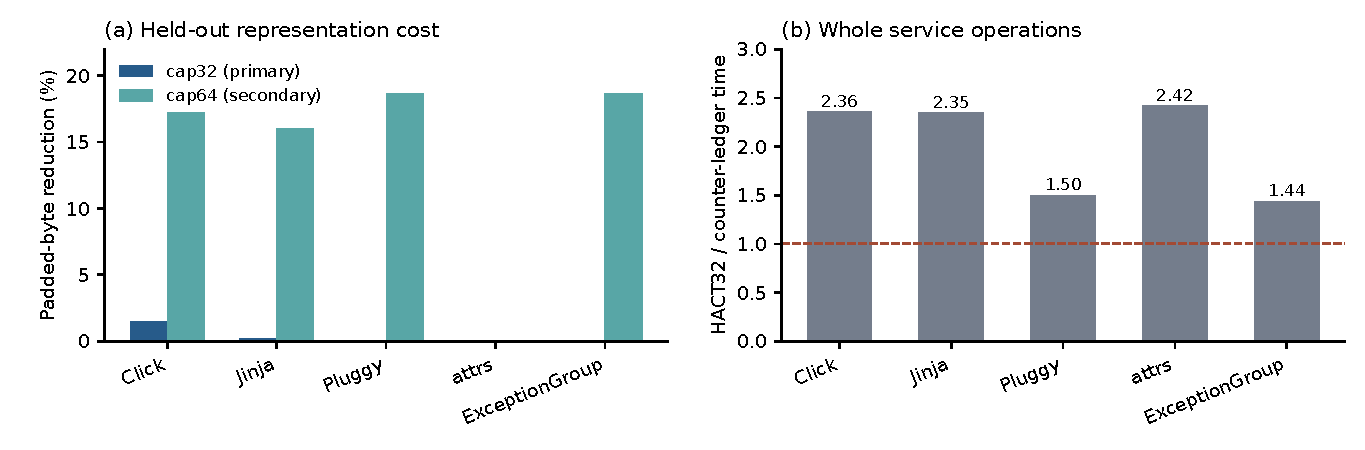
\includegraphics[width=.96\textwidth]{figures/v11_boundaries.pdf}
\caption{Different endpoints lead to different adoption decisions.
Left: primary and prespecified secondary held-out padded-byte savings.
Right: original instrumented precompiled service time of primary HACT divided by the
maintained-counter ledger; values above one are slower. Packaging is
UNKNOWN under resource admission and is not plotted as zero.}
\label{fig:v11-boundaries}
\end{figure*}

\subsection{Controlled dispatch-shift transfer}
The new campaign contains 36 complete suite executions and 20,580 check
executions. Six initial ExceptionGroup runs are VOID for cost analysis:
the profiler observed an ignored build-generated version module absent from
the frozen tracked-source inventory. Their raw records are retained. A
separate child protocol freezes that module before rerunning all six
predeclared schedules, without changing tests, seeds, layouts or endpoints.
The resulting admitted comparison has 30 executions and 19,968 checks over
five projects; it does not silently reclassify the original exclusions.
All admitted runs retain the original registry and status counts, including
attrs' environment-related failures.

\begin{table}[t]\centering\footnotesize
\caption{Primary cap32 padded-byte reduction (\%) under controlled dispatch
shifts relative to historical compact selection. Ranges span the three
fixed seeds; negative values are losses. No refitting.}
\label{tab:v12-shifts}
\begin{tabular}{@{}lrr@{}}\toprule
Project & File groups & Individual items\\\midrule
Click & -4.85 to -3.33 & -9.01 to -8.94 \\
Jinja & 0.15 to 0.17 & -0.12 to -0.07 \\
Pluggy & 0.00 & 0.00 \\
attrs & 0.00 & 0.00 \\
ExceptionGroup & 0.00 & 0.00 \\
\bottomrule\end{tabular}\end{table}

Against the historical selected comparator, file-group shuffling gives
three primary wins, nine ties and three losses; item shuffling gives zero
wins, nine ties and six losses. The comparison unit here is a scheduled
process, not an independent project. The small Jinja file-group gain survives,
whereas Click loses under both shifts. The three ties are projects whose
primary selection did not change. This directly limits the inference from
the repeated-pattern holdout. Every seed, all four frozen layouts, the
original compact comparison and secondary cap64 prices are retained in
the artifact. Neither the intervention nor the analytical witness identifies
natural deployment prevalence or a causal higher-order benefit.

\subsection{Service costs with byte observers disabled}
The separate ablation completes 240 arm executions: ten held-out traces,
three repeats and eight arms. All 10,080 raw-oracle/common-codec answer
checks agree; the two complete Packaging traces remain UNKNOWN under the
unchanged service budget. Table~\ref{tab:v12-observer} compares the same
primary layout to the maintained-counter ledger within each new timing block.

\begin{table}[t]\centering\footnotesize
\caption{Observer ablation. Disabled columns are mean case-median operation
times (ms); ratios compare HACT32 with counters in the same campaign.
Inst.=original instrumentation; off=byte observers disabled.}
\label{tab:v12-observer}
\begin{tabular}{@{}lrrrr@{}}\toprule
& \multicolumn{2}{c}{Observers off (ms)} & \multicolumn{2}{c}{HACT/counter}\\
Project & Counter & HACT32 & Inst. & Off\\\midrule
Click & 137.9 & 429.2 & 2.16 & 3.11 \\
Jinja & 140.3 & 446.1 & 2.23 & 3.18 \\
Pluggy & 23.0 & 37.1 & 1.45 & 1.61 \\
attrs & 261.3 & 924.9 & 2.64 & 3.54 \\
ExceptionGroup & 20.3 & 39.0 & 1.43 & 1.92 \\
\bottomrule\end{tabular}\end{table}

Removing observational serialization reduces absolute service time but
does not reverse the comparison. Primary HACT is slower than counters
in every paired timing block under both instrumentation states. With
observers disabled, the project ratios of mean case medians range from
1.61 to 3.54; individual paired-block ratios range from
1.135 to 4.630. These are descriptive host-specific
ranges, not confidence intervals. The disabled variant retains functional
packet serialization, evidence digests, record copies, validation, caches
and codec round trips. It is a controlled prototype ablation, not an optimized
production implementation. The negative service result therefore survives
the identified observer-cost confound for this demand.


% Generated by experiments_v13.report from audited retained v13 numbers.
\subsection{Exact scoring interfaces and conditional adoption}
Proposition~\ref{prop:summary-span} separates two requirements:
retaining enough information to fit a new layout, and scoring a frozen
catalogue. On all 90 three-block partitions of six checks, an exact
rational calculation gives rank 16 for the constant and fifteen pairwise
same-window features, rising to 17 after appending the grouped-versus-flat
paired score. A single additional score feature suffices for this fixed
comparison. The rank calculation verifies the scoring statement; the
earlier global-optimum theorems supply the stronger optimization obstruction.

The independent literal-tree scorer agrees with the paired implementation
and structural envelope in 247,680 comparisons: all 2,752 labeled unordered
six-leaf trees against flat, across all 90 complete three-window partitions.
The checks include arbitrary display orders; four-leaf regressions also
enumerate every feasible width/window-count combination. These are exact
analytical conformance checks, not new software projects.

For the complete-epoch witness at the implemented prices, the grouped
layout saves an expected 32 bytes under $P$ and loses 102.4 under $Q$.
Its paired support interval is $[-3328,256]$, of width 3,584 bytes;
bounding both whole costs separately gives width 22,784. Their squared
width ratio is approximately 40.41, a bound-dependent sample-complexity
comparison, not measured task acceleration.

We fix the two layouts, $\delta=0.05$, zero shift, a 1,000-epoch horizon
and 3,684 additional pre-horizon installation bytes before a seeded
synthetic calibration study. Twenty seeds per law use nested prefixes of
100,000 draws. Table~\ref{tab:v13-adoption} reports conditional-adoption
counts for Equation~\eqref{eq:adoption-lower}; whole-cost bounds use the
same observed paired means and installation ledger. The direct streaming
API agrees with the intended positive scenario and retains the incumbent
when the declared TV radius rises to 0.01. No population significance or
empirical confidence coverage is inferred from these twenty seeds.

\begin{table}[t]\centering\small
\caption{Synthetic conditional adoption counts. Repeated prefixes are
dependent within seed. Under $Q$, neither bound adopts at any listed size.}
\label{tab:v13-adoption}
\begin{tabular}{@{}rrrr@{}}\toprule
Calibration $m$ & $P$: paired & $P$: whole & $Q$: paired\\\midrule
100 & 0/20 & 0/20 & 0/20\\
1,000 & 0/20 & 0/20 & 0/20\\
10,000 & 1/20 & 0/20 & 0/20\\
100,000 & 20/20 & 0/20 & 0/20\\
\bottomrule\end{tabular}
\end{table}

Even with infinite calibration and no installation charge, a mean saving
of 32 bytes cannot make this lower bound positive for
$\rho\ge32/3584=1/112$. This is the limit of this conservative certificate,
not a sharp minimax drift tolerance or an estimate of software-workload drift.
All five admitted public-project rows remain $\UNKNOWN$: repeated
snapshots and controlled schedule interventions supply neither the required
independent natural calibration nor an externally justified deployment TV
bound. Packaging's resource exclusion is retained separately. This new
analysis neither changes the historical 3/18/9 shift outcomes nor establishes
a service advantage over the maintained-counter ledger.

% Generated by experiments_v14.report from audited retained observations.
\subsection{A stronger symmetric-model baseline}
The exact size-state solver matches independent all-tree enumeration in
70 combinations of size, fanout and flush width, totaling 74,245 feasible
tree comparisons for $n\le6$. Its reference averages actual completion
permutations rather than importing the hypergeometric formula. Additional
regressions cover every small positive batch-size composition, arbitrary
leaf orders, three packet-price regimes and exact reconstruction. This
checks the model-specific global optimum, not the symmetry of software data.

We then fit this baseline to registry size and the declared eight-record
flush only, using canonical semantic order and no training traces.
This retrospective comparison re-encodes the same 25 original executions
and 30 admitted dispatch interventions; it adds no checker execution.
The baseline beats the frozen cap32 full-wave layout on all 15 item-shuffled
traces and loses on all 15 file-group traces. Table~\ref{tab:v14-symmetry}
uses per-project ratios of summed bytes across three retained seeds per
policy. Positive values mean fewer padded bytes than the frozen full-wave
layout. Policy/seed repetitions are not independent projects.

\begin{table}[t]\centering\small
\caption{Exact symmetric-model baseline versus frozen full-wave cap32.
Savings (\%) retain both successful and unfavorable dispatch policies.}
\label{tab:v14-symmetry}
\begin{tabular}{@{}lrrr@{}}\toprule
Project & Checks & Item shuffle & File groups\\\midrule
click & 761 & +15.67 & -7.29\\
jinja & 909 & +7.22 & -11.50\\
pluggy & 124 & +5.28 & -15.77\\
attrs & 1,432 & +8.26 & -23.77\\
exceptiongroup & 102 & +7.00 & -10.60\\
\bottomrule\end{tabular}
\end{table}

On the original repeated-order holdouts, the model baseline instead costs
21.26--62.13\% more than frozen full-wave selection. Packaging remains
outside the 2,048-check fitting budget. These outcomes identify complementary
regimes: size-only topology is a strong control for dispersed completions,
while learned locality can matter for structured groups. Shuffled dispatch
does not prove exchangeable completion times. The baseline's smaller packet
cost in one controlled regime does not overturn the counter-ledger service
result or establish a net lifecycle benefit on natural consumer demand.


\section{Related Work}\label{sec:jrelated}
Test prioritization, regression selection and self-adjusting computation
already optimize which work is executed and recomputed~\cite{rothermel,ekstazi,acar,build}.
HACT leaves the approved registry and check schedule under the runner's control; its local pass
requires the entire declared contract. It does not reproduce regression
selection systems or assert superiority over them.

Graham, Li and Yao price every touched ancestor in batch-update key trees
and derive structural bounds and an $O(n)$ solver for their independent
Bernoulli replacement model~\cite{graham2007}. Thus touched-ancestor
pricing and cardinality-based tree DP precede HACT. Our fixed-size
without-replacement batches, affine capped packets and cold-build charge
define the exact baseline in Section~\ref{sec:symmetry}; the information
separation concerns correlated laws outside that symmetric regime.
Alphabetic-tree optimization supplies the fixed-order dynamic program
\cite{alphabetic}. Pairwise seriation supplies an established ordering
proposal~\cite{atkins}. Dasgupta's objective charges pairwise similarities
through hierarchical cluster sizes~\cite{dasgupta}; constrained hierarchical
clustering explicitly uses three-hypergraph objectives~\cite{hyperhierarchy}.
Balanced and hierarchical hypergraph partitioning likewise prices collective
communication~\cite{hyperpartition}. HACT's affine arity prices, every-touched-node
objective, unrestricted shapes and lifecycle costs differ from these models.
Their hardness or approximation guarantees do not transfer automatically.

Authenticated workload-adaptive structures optimize access and proof
costs~\cite{hmt}. HACT's local binding capsules are not membership proofs,
signatures or attestations. Verification-first AI engineering and
trace-assurance frameworks govern actions and checks~\cite{aiware,traceassurance};
HACT isolates the representation that accumulates after such checks.
Its optional migration policies specialize established switching-cost expert
methods; the full historical manuscript retains their assumptions and
negative comparisons. Batched telemetry and ordinary compression remain
required controls, not techniques displaced by a tree.
Independent calibration followed by simultaneous risk testing is an
established framework~\cite{learntest}. Our adoption rule specializes this
principle to differences of verification-packet costs, with semantic
coverage cancellation, declared completion support and separately priced
installation. Its Hoeffding and total-variation arguments are standard.

\section{Threats to Validity and Deployment Guidance}
The packet objective is additive and format-specific. Byte constants,
refresh batching and fixed execution schedules constrain external validity.
The theorem establishes a worst-case information limit, not that most
workloads need higher moments. The new refinement is exact only in its
declared restricted class and to the reference DP's numerical precision.
A different proposal budget or order can produce different results.
The conditional adoption rule does not repair unknown sampling or drift.
The archived software cohorts do not establish its IID calibration and
deployment-radius assumptions. Its synthetic validation demonstrates
conformance within a specified model; it adds no independent software cases.
The exchangeable optimum is exact for its law, not for arbitrary completion
traces. Canonical labels, rather than learned locality, define its empirical
baseline. Its item/file reversal and original-holdout losses preclude
universal superiority. The retrospective baseline comparison is descriptive;
dispatch intervention is not a test establishing exchangeability.

The convenience sample has six small Python projects, one excluded from
fitting. The five admitted projects repeat completion patterns across
original splits, establishing repeatability. Dispatch interventions probe
artificial schedule changes; neither cohort establishes natural workflow
generalization. Packaging supplies 89.0\% of the initial executions;
the admitted compiler cohort has 25 runs and 16,640 checks. Historical
replays, normal-suite repeats and transplanted regressions remain distinct
sampling units. Environment incompatibilities remain recorded and are not
automatically attributed to upstream defects.

Controlled fixed-group demand favors maintained counters. A useful tree
region requires independently justified delivery or aggregation savings
that repay lifecycle costs. Equal codec bytes establish conformance.
No live-model, token-billing or physical-WAN benefit is inferred from
these local measurements.

The safety result assumes trusted immutable checking and atomic local
fencing. Tests do not certify test adequacy, and a report file is not an
atomic external commit. The mathematical conclusions are conditional on the stated model and
information interface, and empirical conclusions are limited to the recorded
cohort and demand. These limits determine the contribution's external validity.

\section{Conclusion}
Joint completion events contain optimization information that exact pairwise
summaries can irretrievably lose. Under exchangeability, however, cardinality
alone suffices for a global optimum without learning. Adaptive HACT separates
these regimes while keeping adaptive representations outside semantic
authority. Its exact symmetric baseline and bounded full-wave refiner expose
complementary strengths on dispersed and grouped completions; the evaluation
preserves the unfavorable cases and strong ledger controls.
The adoption rule quantifies when independent paired evidence can cover
sampling uncertainty, a declared shift allowance and installation bytes.
The practical implication is conditional: keep semantic authority fixed,
retain full completion sets when fitting the stated packet objective, and
validate under the changes expected in deployment. The controlled dispatch
losses reject universal transfer, and the observer-disabled service comparison
supports maintained counters for the evaluated requests. Retain the incumbent
when independent lifecycle evidence does not justify a change.

\section*{Data and Code Availability}
The accompanying v14 artifact contains code, versioned observations,
exact references and independent audits. The historical repository link is withheld in this blinded manuscript.
The accompanying review artifact supplies the referenced observations.
The release manifest binds source and PDF bytes; it is not a signature.
The artifact includes the full historical analysis, raw execution receipts,
a reproduction guide and a claim-to-evidence map. A hash-bound offline
archive restores the original observation paths before manifest verification
and independent audits; it preserves every recorded exclusion and outcome.
\section*{Acknowledgments}
OpenAI Codex (October 2026) assisted with prose throughout the article,
the proofs and analytical examples in Sections III--V, the TikZ source
of Figure~\ref{fig:journal-architecture}, and the experiment, reference and
audit code supporting Sections VI--VII. Its use included drafting,
derivation, implementation, experiment execution and automated checks.
The separately implemented checks reduce shared-code risk; they are
AI-assisted checks, not independent human peer review. The authors retain
responsibility for the article's content, correctness and citations.

% Verified source entries, restricted to citations in journal.tex and its inputs.
\begin{thebibliography}{99}
\sloppy
\bibitem{swebench} Carlos E. Jimenez, John Yang, Alexander Wettig, Shunyu Yao, Kexin Pei, Ofir Press, and Karthik Narasimhan.
\newblock SWE-bench: Can Language Models Resolve Real-World GitHub Issues?
\newblock \emph{International Conference on Learning Representations}, 2024.
\newblock \url{https://arxiv.org/abs/2310.06770}.

\bibitem{sweagent} John Yang, Carlos E. Jimenez, Alexander Wettig, Kilian Lieret, Shunyu Yao, Karthik Narasimhan, and Ofir Press.
\newblock SWE-agent: Agent-Computer Interfaces Enable Automated Software Engineering.
\newblock arXiv:2405.15793, 2024.
\newblock \url{https://arxiv.org/abs/2405.15793}.

\bibitem{openhands} Xingyao Wang et al.
\newblock OpenHands: An Open Platform for AI Software Developers as Generalist Agents.
\newblock arXiv:2407.16741, 2024.
\newblock \url{https://arxiv.org/abs/2407.16741}.

\bibitem{aiware} Qinghua Lu, Ahmed E. Hassan, David Lo, and Thomas Zimmermann.
\newblock Engineering Agentic Systems: Toward Verification-First AIware Engineering.
\newblock \emph{IEEE Software}, 43(5):22--29, 2026.
\newblock \url{https://doi.org/10.1109/MS.2026.3697911}.

\bibitem{traceassurance} Ciprian Paduraru, Petru-Liviu Bouruc, and Alin Stefanescu.
\newblock A Trace-Based Assurance Framework for Agentic AI Orchestration: Contracts, Testing, and Governance.
\newblock arXiv:2603.18096, March 2026.
\newblock \url{https://arxiv.org/abs/2603.18096}.

\bibitem{alphabetic} Hirendu Vaishnav and Massoud Pedram.
\newblock Alphabetic Trees: Enumeration and Optimization with Applications to VLSI Design.
\newblock Undated author-hosted manuscript, Sections 4.1--4.4.
\newblock \url{https://www.mpedram.com/Papers/alp-trees-journal.pdf}.

\bibitem{hoeffding} Wassily Hoeffding.
\newblock Probability Inequalities for Sums of Bounded Random Variables.
\newblock \emph{Journal of the American Statistical Association}, 58(301):13--30, 1963.
\newblock \url{https://doi.org/10.1080/01621459.1963.10500830}.

\bibitem{rothermel} Gregg Rothermel, Roland H. Untch, Chengyun Chu, and Mary Jean Harrold.
\newblock Prioritizing test cases for regression testing.
\newblock \emph{IEEE Transactions on Software Engineering}, 27(10):929--948, 2001.
\newblock \url{https://doi.org/10.1109/32.962562}.

\bibitem{ekstazi} Milos Gligoric, Lamyaa Eloussi, and Darko Marinov.
\newblock Practical regression test selection with dynamic file dependencies.
\newblock \emph{Proceedings of ISSTA}, 2015.
\newblock \url{https://users.ece.utexas.edu/~gligoric/papers/GligoricETAL15Ekstazi.pdf}.

\bibitem{acar} Umut Acar, Guy Blelloch, Matthias Blume, Robert Harper, and Kanat Tangwongsan.
\newblock A Library for Self-Adjusting Computation.
\newblock \emph{Electronic Notes in Theoretical Computer Science}, 148:127--154, 2006.
\newblock \url{https://doi.org/10.1016/j.entcs.2005.11.043}.

\bibitem{build} Andrey Mokhov, Neil Mitchell, and Simon Peyton Jones.
\newblock Build Systems \`a la Carte.
\newblock \emph{Proceedings of the ACM on Programming Languages}, 2(ICFP), Article 79, 2018.
\newblock \url{https://doi.org/10.1145/3236774}.

\bibitem{atkins} Jonathan E. Atkins, Erik G. Boman, and Bruce Hendrickson.
\newblock A Spectral Algorithm for Seriation and the Consecutive Ones Problem.
\newblock \emph{SIAM Journal on Computing}, 28(1):297--310, 1998.
\newblock \url{https://doi.org/10.1137/S0097539795285771}.

\bibitem{dasgupta} Sanjoy Dasgupta.
\newblock A cost function for similarity-based hierarchical clustering.
\newblock \emph{Proceedings of STOC}, pages 118--127, 2016.
\newblock \url{https://doi.org/10.1145/2897518.2897527}.

\bibitem{hyperhierarchy} Vaggos Chatziafratis, Rad Niazadeh, and Moses Charikar.
\newblock Hierarchical Clustering with Structural Constraints.
\newblock \emph{Proceedings of ICML}, PMLR 80:774--783, 2018.
\newblock \url{https://proceedings.mlr.press/v80/chatziafratis18a.html}.

\bibitem{hyperpartition} P\'al Andr\'as Papp, Georg Anegg, and A. N. Yzelman.
\newblock Partitioning Hypergraphs is Hard: Models, Inapproximability, and Applications.
\newblock \emph{Proceedings of SPAA}, 2023.
\newblock \url{https://doi.org/10.1145/3558481.3591087}.

\bibitem{hmt} Ziheng Shangguan, Aviv Yaish, and Dahlia Malkhi.
\newblock Authenticated Data Structures for Dynamic Workloads.
\newblock arXiv:2608.25206v1, August 2026.
\newblock \url{https://arxiv.org/abs/2608.25206v1}.
\bibitem{learntest} Anastasios N. Angelopoulos, Stephen Bates, Emmanuel J. Cand\`es,
Michael I. Jordan, and Lihua Lei.
\newblock Learn then Test: Calibrating Predictive Algorithms to Achieve Risk Control.
\newblock arXiv:2110.01052v5, 2022.
\newblock \url{https://arxiv.org/abs/2110.01052v5}.
\bibitem{graham2007} Ronald L. Graham, Minming Li, and Frances F. Yao.
\newblock Optimal Tree Structures for Group Key Management with Batch Updates.
\newblock \emph{SIAM Journal on Discrete Mathematics}, 21(2):532--547, 2007.
\newblock \url{https://doi.org/10.1137/06064929X}.
\end{thebibliography}

\end{document}
